\section{Introduction}\label{s:intro}

%\radhika{Alternate intro: mostly just changed the flow of certain points, removed some that might be better suited in related work, and made some more concrete/specific. /*}

%lots of scheduling algorithms proposed. scheduling used in private wans. seems clearly beneficial.

% Although router vendors have, over the years, implemented certain schemes (such as strict priorities, round-robin for fair queueing, and active queue management~\cite{cisco-qos}), they are often not enabled, or used effectively, by the public network operators.\footnote{Private WANs are different, and are not the focus of our work. Being owned by the content providers themselves, they have been successful in exploiting the benefits of scheduling~\cite{swan, b4, bwe}.}  
% This is primarily due to the challenging position of public network operators, where each of their customers may desire diverging, and often incompatible, features. While Netflix might prefer enforcing fairness across its video traffic, Amazon might prefer prioritizing its interactive web store traffic over the long-lived AWS transfers.
% %For example, while enabling fair queueing in the routers would benefit short interactive flows competing with bulk transfers, it may penalize flows bundled within a single VPN tunnel by allocating them smaller than their fair share of bandwidth \radhika{might need to change this example}. 
% %Similarly, while enabling an AQM scheme might reduce the queuing delay in the absence of a BBR flow, it may severely penalize non-BBR flows that compete with BBR. (include if we find a citation). 
% %\radhika{something about not knowing how to apply policies across customers}
% %\radhika{similar issue arises with our bundler too...}.
% Thus, due to limited visibility into their customers' traffic, network operators cannot choose policies that can appease them all.

% Different content providers in the Internet might benefit from different scheduling policies. For example, Netflix might prefer enforcing fairness across its video traffic, while Amazon might prefer prioritizing its interactive web store traffic over the long-lived AWS transfers. The public network operators, however, have neither enough visibility into the  traffic to choose the desired policies, nor enough incentives to enforce them.\footnote{The case for private WANs is different, since they are owned by a single entity, and have, thus, been successful in exploiting the benefits of scheduling~\cite{swan, b4, bwe}.} \radhika{say something about deals}

% An individual customer can, on the other hand, choose appropriate policies for the \emph{component flows} within its own traffic as per its own requirements. 
% %; that is, scheduling policy is easier to express at the edge. 
% Consider examples such as traffic between different campuses of an organization, or a large content provider (\eg Netflix) and a network with many clients (e.g., a regional ISP), or an organization using an external service (\eg Dropbox), and so on. In each of these scenarios the sender has enough information to unilaterally choose a scheduling or queue management policy for its component flows (such as prioritizing flows based on applications, enforcing fair queueing, or using AQM to bound delays). However, these policies are effective only when enforced on congested links in a flow's path that experience a queue build-up, and such links are often outside the control of the individual customers~\cite{inferring-interdomain-congestion}. 

The vast literature on scheduling and queue management policies~\cite{diffserv, fair-queueing, sfq, pie, CoDel, fifoplus, virtualClocks, csfq, drr, red, ecn} has demonstrated their benefits.
On many Internet paths, however, content providers and end users have been unable to enjoy these benefits.

Internet content providers may desire such policies for their traffic. For example, a video streaming company might benefit from weighted fair queueing across its video traffic to its many different users sharing a bottleneck, and web sites might want to prioritize  interactive web traffic (e.g., e-commerce) over the bulk file transfers. However, such policies are effective only when enforced on bottleneck links that experience a queue build-up, and such links are often outside the control of individual content providers~\cite{inferring-interdomain-congestion, isp-throttle-1, isp-throttle-2, isp-throttle-3}. Content providers are therefore unable to apply desired policies to their traffic in such settings. 

ISPs, on the other hand, do control the bottleneck links in their carrier networks to enforce different scheduling and queue management policies. However, they neither have enough visibility into their customers' traffic to choose desired policies, nor enough incentives to enforce them.\footnote{The case for private WANs is different, since they are owned by a single entity, and have, thus, been successful in exploiting the benefits of scheduling~\cite{swan, b4, bwe}. Our focus is public networks.} Large customers might be able to negotiate deals with certain carriers to enforce specific policies~\cite{att-qos}. However, it might not be possible to negotiate such deals with \emph{all} carriers in the traffic's path, and content providers may wish to keep their policies confidential from downstream ISPs.
%(especially a small last-mile carrier that is likely to be the bottleneck, and that may not even possess switches equipped with required features). 
%Even if this was somehow made possible, the customers would have no way of knowing whether their policies were enforced as desired, and they would be left at the mercy of these individual ISPs.
%, they have no way of knowing whether it was done appropriately. 

%So to summarize, while customers may not have enough control over the queued-up links in the network to effectively enforce their desired policies, the ISPs may not have enough incentives or enough visibility into the traffic to do so. 
To reduce a content provider's dependence on the ISPs with respect to how its traffic is managed, we attempt to bring the provider's traffic under its own control by \emph{moving the queues that its traffic would build at a downstream bottleneck to the provider's edge}. Our approach allows the content provider to enforce its desired traffic management policies across traffic that share common sender and receiver domains.
%(as described in \S\fc{X}). 
The natural question that arises is, how can the queues be ``moved''? This is the primary focus of our work. 

We observe that the \emph{component flows} in traffic from a given sender's domain, destined for the same downstream domain, are likely to share common bottlenecks within the network, as in Figure~\ref{fig:deploy:arch}. Examples include large amounts of traffic between a content provider (\eg Amazon, Google, etc.) and a network with many clients (e.g. an enterprise), between two different campuses of an organization, between collaborating institutes, and so on. By (i) aggregating such component flows into a single \emph{bundle} at the sender's egress, and (ii) controlling the outgoing rate of this bundle to match its bottleneck rate in the network, we can effectively \emph{move} the queues built by the traffic in the bundle, from within the network, to the sender's egress itself. 
%\radhika{is the last sentence too long / hard to understand? suggestions for fixing it?} 
\begin{figure*}[t]
    \centering
    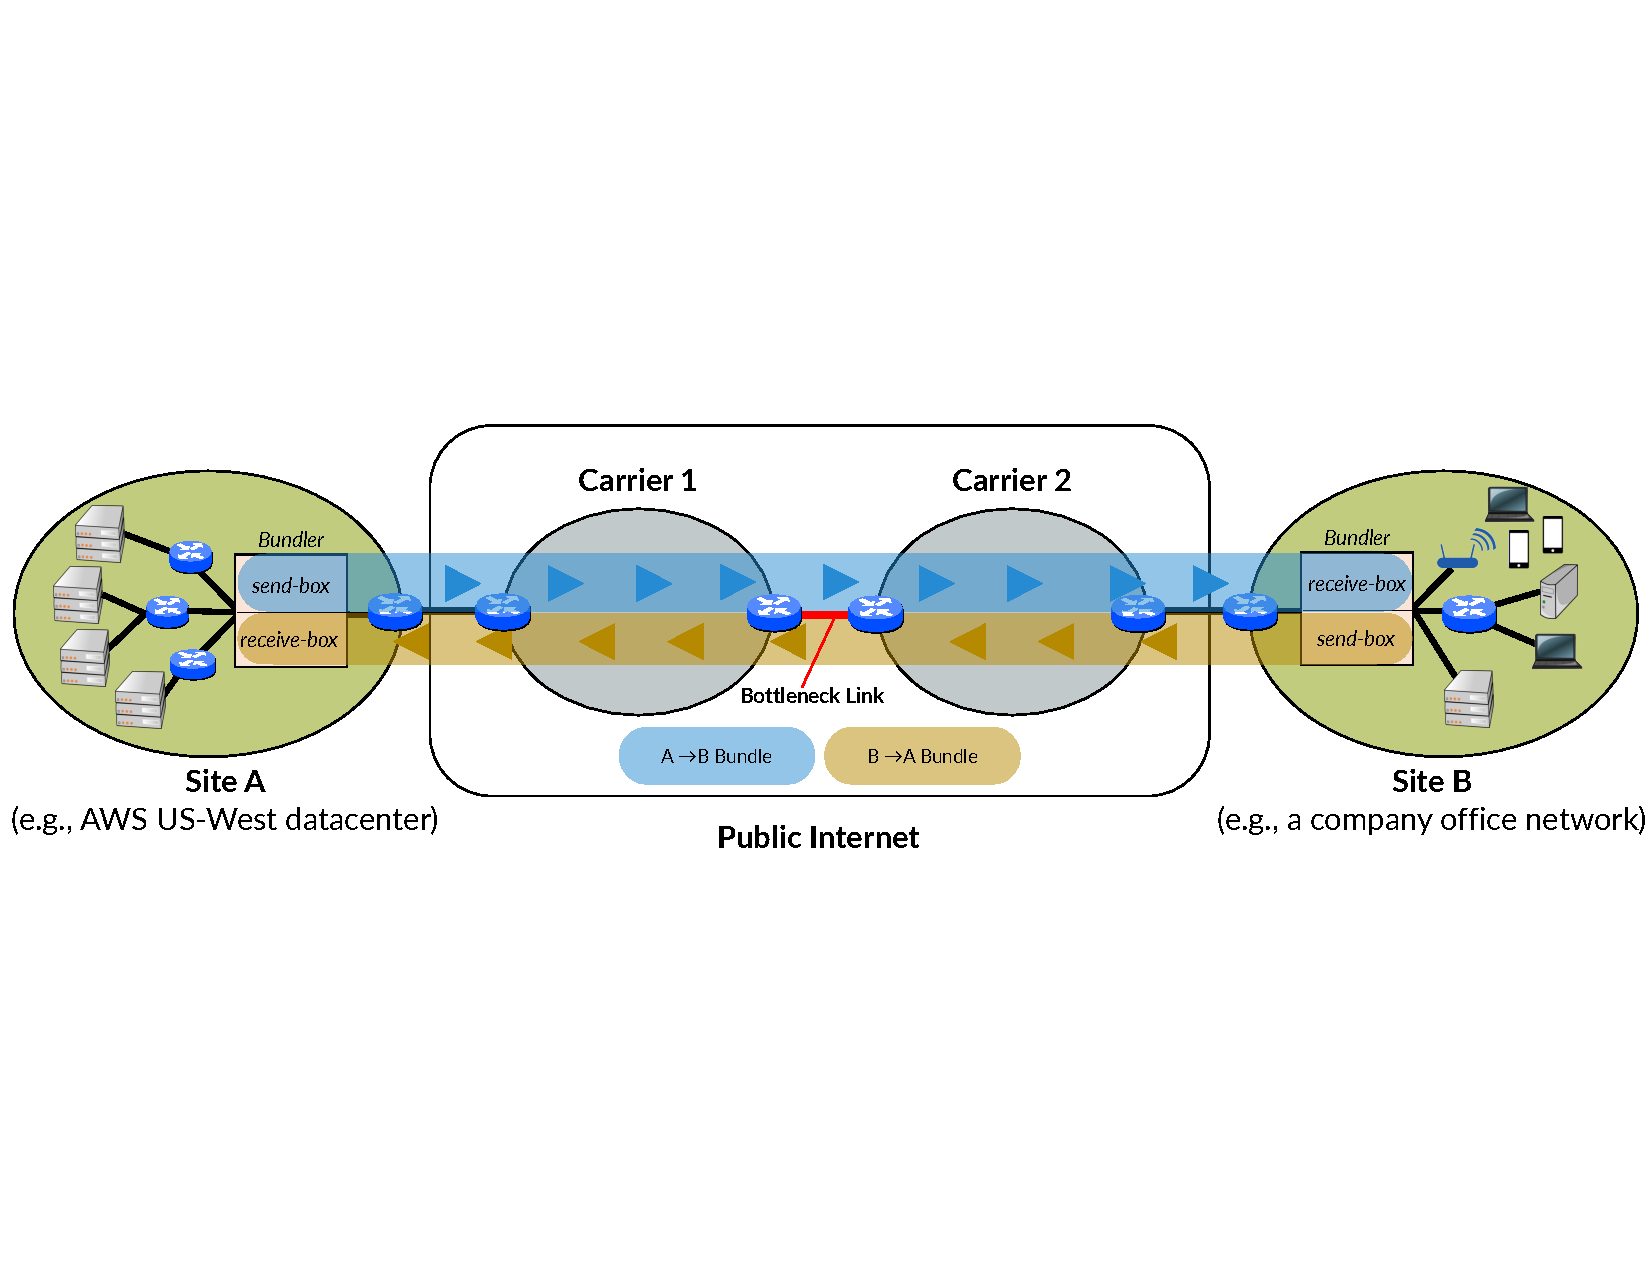
\includegraphics[width=\textwidth]{img/deployment-arch.pdf}
    \caption{An example deployment scenario for \name. 
    The \inbox sits at the sending domain's egress and \outbox sits at the receiving domain's ingress. All traffic between the two boxes is aggregated into a single bundle. The \inbox schedules the traffic within the bundle according to the policy the sending domain specifies (\S\ref{s:design}).
    %Bottleneck links between the \inbox and the \outbox are shown in red.
    %The solid lines depict links used by the traffic in the bundle, while the dotted lines represent other possible links. 
    }\label{fig:deploy:arch}
\end{figure*}

%We further note that middleboxes are now prevalent in the Internet architecture~\cite{aplomb}. They are often deployed at the egress and ingress of a network domain, to ensure traffic transits them for intrusion detection, packet inspection, filtering etc. They thus provide an effective vantage point for aggregating and managing traffic. 
We propose a new type of middlebox, called \name, that (1) aggregates the traffic at \reword{the content provider's} egress into appropriate bundles, (2) does rate control for each bundle to move the corresponding queues from within the network to itself, and (3) applies scheduling and AQM policies within each bundle. 

%\radhika{add a few lines on \name's high level architecture.} 
%\fc{is it not bad to bring up the two-box design here if we don't justify it until later?}
\name is made up of a pair of middleboxes: a \emph{\inbox} that sits at the sender's egress and a \emph{\outbox} that sits at the receiver's ingress. A \emph{bundle} is a group of flows traversing the same \inbox{}-\outbox{} pair. The bulk of \name's functionality resides at the \inbox, which coordinates with the \outbox to measure congestion signals, such as the round-trip time, and the rate at which packets are received. These signals are used by a congestion control algorithm (requiring certain properties described in \S\ref{s:design}) that runs at the \inbox and computes appropriate sending rates for each bundle. The sending rates are computed such that the queuing induced by the bundled traffic within the network is low and is incurred at the \inbox instead, while ensuring that the bottleneck link on the path remains fully utilized. 
 
We introduce a lightweight method for the coordination between the \inbox and the \outbox, which does not require any per-flow state, nor any modifications to the packets traversing the \name boxes. Our approach only requires introducing the \name boxes at the content provider's edge, and requires no changes to the end hosts or to the routers in the network. 
 
Note that our goal is to perform scheduling and queue management only on the traffic within the same bundle. We do not attempt to control traffic across different bundles. Furthermore, as we will discuss in \S\ref{s:deploy}, there may be instances where \name does not improve performance for the bundled traffic, and falls back to the status quo performance. Despite these limitations, we believe that our work, provides a deployable solution for enabling some of the benefits of scheduling and queue management in the Internet from the edge of the content provider's network.
 
We make the following contributions:
\begin{enumerate}
     \item A light-weight, scalable and deployable design of \name that does congestion control on aggregated traffic to move queues to the content provider's edge (\S\ref{s:design}).  
     \item A novel low-overhead protocol-agnostic technique for measuring signals for congestion control between the \pair, that does not make any changes to the packet headers (\S\ref{s:measurement}). We evaluate our measurement strategy across a variety of RTTs and link bandwidths in \S\ref{s:measure:microbench}. 
     \item A prototype implementation of \name (\S\ref{s:impl}).
     \item Evaluation of our prototype implementation on a wide variety of emulated scenarios with a demonstration of performance benefits achieved from scheduling traffic via \name (\S\ref{s:eval}).
     In a scenario with self-inflicted scheduling overhead, \name achieves 33\% lower median slowdown.
     %\item The design and implementation of a \name, including a novel method of collecting congestion control information and enforcing the decisions of a rate control algorithm on traffic aggregates, which \emph{moves} the queues from the bottleneck in the network to the customer's edge.
     %\item An evaluation of the benefits of scheduling and queue management for traffic aggregates, compared to both the status quo (FIFO) and an idealized deployment where bottleneck queues deploy the desired policy.
 \end{enumerate}

 %\radhika{should i move it up by 2 paragraphs (i.e. right after the 3 points)?} 

%The rest of the paper dives into the details of how we design, implement and evaluate \name, and is organized as follows:
%We begin the rest of this paper by discussing some related work in \S\ref{s:related}. We then discuss our design choices, along with the favorable operation regime for \name in \S\ref{s:design}. We detail our novel \inbox and \outbox coordination methodology for collecting congestion signals in \S\ref{s:measurement}, and describe our prototype implementation in \S\ref{s:impl}. 
%\S\ref{s:design} describes the \name architecture and the various trade-offs we considered when designing it.  
%\S\ref{s:measurement} describes our novel approach for gathering measurements from the network to do rate control at the \name in order to move the bottleneck. 
%\S\ref{s:impl} describes our prototype implementation. 
%Finally, in \S\ref{s:eval}, we use our prototype implementation to evaluate the performance benefits of using a \name across a wide variety of emulated scenarios, before concluding in \S\ref{s:concl}.
%\radhika{revise}
%Middleboxes offer a flexible design point, since implementations spanning hardware and software represent numerous options in implementing scalable, yet flexible and sophisticated scheduling policies. 

%Consequently, the emergence of programmable scheduling~\cite{pifo} might also not be a panacea; while it might make it simpler to implement different scheduling policies, their enforcement would remain difficult due to lack of sufficient knowledge about the customers' requirements. 

%On the other hand, even simple policies, such as priority scheduling across a small number of traffic classes, deployed within privately operated wide-area networks, have been shown to provide significant gains in performance~\cite{b4, swan, bwe} \radhika{can we also show some results with priority scheduling in eval?}.  
%, and the deployment of simple scheduling policies in privately ~\cite{b4, bwe, swan} clearly indicates the benefits of 

%individual customers can choose, but can't enforce scheduling at edge. makes most sense to do it an congested routers, out of their control.

\cut{
\radhika{*/ Old intro:}


Most Internet paths today employ first-in, first-out (\emph{FIFO}) scheduling \radhika{I think they might also do some coarse-grained priorities. Let's not make this our first sentence, unless we are absolutely sure.}. 
However, traffic could benefit from different scheduling algorithms.
The bottleneck link, where congestion occurs and therefore where scheduling is the most useful, is often at the edge of a network, whether an individual device or an autonomous system~\cite{inferring-interdomain-congestion} \radhika{the last part of this sentence not super clear to me.}. 
As a result, deploying scheduling algorithms on one's own routers is of limited utility; often, the congestion occurs in a router outside of one's control.
Unfortunately, networks have proven difficult to evolve; although router vendors have, over the years, implemented other scheduling algorithms (such as fair queueing~\cite{fair-queueing}), operators often do not enable these features.
Thus, the emergence of programmable switching~\cite{p4} is not a panacea; while it might now be simpler to implement scheduling policy, it remains difficult to see deployment \radhika{P4 does not ease deployment of scheduling algorithms.}.
Meanwhile, in privately operated wide-area networks, operators have used scheduling in the core to reap significant gains~\cite{b4, bwe, swan}. 
Clearly, the use of scheduling policy is beneficial.

Why, then, are operators hesitant to deploy new scheduling policies on congested routers? 
First, scheduling policy can be difficult to configure, and poor configurations can cause significant performance degradation~\cite{nanog-discussion}.
Second, the position of operators in the public Internet is a challenging one, as each of their various customers may desire diverging (often incompatible) features. For example, due to the prevalence of VPN tunnelling, enabling fair queueing in routers may penalize flows bundled within a VPN tunnel.
Thus, operators cannot see the full picture, and cannot offer scheduling that will appease any one customer.

Crucially, however, \emph{individual customers} can often choose a policy that suits their needs; that is, scheduling policy is easier to express at the edge. 
Examples include: traffic between different datacenters over the public Internet; traffic between campuses of an organization; traffic between collaborating universities or companies; traffic between a large content provider (\eg Netflix) and a network with many clients (e.g., a regional ISP); large-scale data backups from an organization to an external site (\eg Dropbox); etc. 
In each of these scenarios the sender has enough information to unilaterally choose a scheduling policy for its component connections, but usually lacks the control over the bottleneck link necessary to realize it.

While it may be easier to \emph{express} scheduling policy near the edge, it is not immediately obvious how to \emph{implement} it \radhika{express vs implement distinction might be too subtle for first time readers}. 
Traffic from a domain is naturally comprised of numerous individual connections;
each connection independently probes for bandwidth, detects congestion on its path, and reacts accordingly \radhika{this sentence seems a bit out-of-blue. a connector to previous sentence needed.}.

\radhika{need a brief overview of bundler architecture (maybe the middlebox paragraph that appears later), before diving into technical challenges below.}

We address this challenge in two steps. 
First, we treat the traffic from multiple component connections as a \emph{single aggregate}, \ie as a router would view them \radhika{what does the last part of the sentence mean?}. We decide a combined sending rate for the aggregate. Then, inside the aggregate, we enforce a scheduling policy among the component flows. 
In other words, we decouple the aggregate rate decision from the scheduling policy.
This approach, which we call {\em aggregate traffic control}, therefore has two technical challenges:
\begin{enumerate}
    \item {\bf Congestion control.} At what combined rate should the traffic aggregate send packets? This depends on network conditions at the bottleneck, which the traffic aggregate cannot directly observe.
    Fortunately, this is exactly the question answered by congestion control algorithms; they take as input measurements of network conditions -- RTT, sending rate, receiving rate, etc -- and yield as output a rate at which to send packets.
    Furthermore, since the traffic aggregate as a whole determines the sending rate, this approach causes component flows share congestion information.
    Thus new flows can discover and adapt to their path's congestion conditions much more quickly, which is particularly beneficial for short flows~\cite{CM}. 
    
    \item {\bf Flow scheduling.} Given a combined rate, in what order should the aggregate transmit packets?  This enables fine-grained scheduling for flows within a traffic aggregate. 
    For example, we can schedule flows based on size (short flows first), application priorities, deadlines, etc.
\end{enumerate}

How should we implement and deploy our approach? 
We note that middleboxes are now prevalent in the Internet architecture~\cite{aplomb}.
The rise of middleboxes allows a new vantage point into flows, since middleboxes are often deployed at natural ``choke points'' \radhika{choke point by definition means a bottleneck -- any other word we can use instead?} in a network to ensure traffic transits them for \eg traffic analysis or intrusion detection.
Middleboxes offer a flexible design point, since implementations spanning hardware and software represent numerous options in implementing scalable, yet flexible and sophisticated scheduling policies.
We therefore propose a new type of middlebox to perform traffic aggregation, which we call a \name.

We make the following contributions:
\begin{enumerate}
    \item The design and implementation of a \name, including a novel method of collecting congestion control information and enforcing the decisions of a congestion control algorithm on traffic aggregates. This method \emph{moves} the queues in the network from the bottleneck to the edge.
    \item An evaluation of the benefits of scheduling for traffic aggregates, compared to both the status quo (FIFO) and an idealized deployment where bottleneck queues deploy a scheduling algorithm.
\end{enumerate}

The rest of this paper is organized as follows: 
\S\ref{s:design} describes tradeoffs in the design of a \name. 
\S\ref{s:measurement} describes our approach to gathering measurements from the network. 
\S\ref{s:impl} describes our prototype implementation. 
\S\ref{s:eval} shows an evaluation of the benefits of \name.


}
\cut{
\begin{outline}
\1 Previously, this approach has required terminating the TCP connection at the middlebox; \ie implementing a TCP proxy.
    \2 TCP proxies are widely used to add congestion control functionality in the network.
    \2 \an{drawbacks of TCP proxies}
        \3 head of line blocking
        \3 implementation complexity
        \3 end-to-end principle
\end{outline}
}
